
\subsection{Problem statement}
The invariant spin axis of a particle involved in betatron oscillations wobbles
about its reference orientation.~\cite[p.~11]{Shatunov} For this reason, the amplitude of the T-BMT equation
solution for the vertical spin vector component:
\begin{align}
s_y &= \sqrt{\bkt{\frac{\w_y\w_z}{\w}}^2 + \bkt{\frac{\w_x}{\w}}^2}\cdot\sin\bkt{\w\cdot t + \phi}\notag\\
&= \sqrt{\bkt{\bar n_y\bar n_z}^2 + \bar n_x^2} \cdot \sin\bkt{2\pi\cdot\nu_s\cdot n_{turn} + \phi},\label{eq:sy_varying_amplitude}
\end{align}
becomes a time-varying function. If a particle's invariant spin axis (as well sa spin tune) varies in
a sufficiently big range, use of a constant parameter harmonic function as a model
for fitting the measured signal will introduce the model specification systematic error.
Errors of this type reflect on the validity of the model parameter estimates, i.e. the frequency estimate,
and hence require analysis.

Spin tune ($\nu_s$) variability is especially problematic in this respect,
since it directly affects the phase of the signal; however, this problem can be solved
by introducing sextupole field elements into the beamlinr, as is described
in section~\ref{sec:sextupole_spin_dec_solution}. For this reason, we will focus on the variation of
$\bar n$ in this section.

\subsection{Simulation}
The simulation setup was as follows: a particle offset from the reference orbit in the vertical direction
by 0.3 mm, is injected multiple times into an imperfect FS-type lattice~\cite{Senichev:Lattices},
in which we suppress spin decoherence caused by vertical plane betatron oscillations
(see section~\ref{sec:sextupole_spin_dec_solution})  by using the corresponding sextupole family.
Machine imperfections are simulated as E+B element tilts about the optic axis.
Imperfections introduced this ways do not perturb the closed orbit (that is,
the reference orbit --- as well as the orbit of the betatron-oscillating particle ---
is the same for every injection.)

Each trial, E+B element tilts are randomly distributed as $\alpha\sim N(\mu_i, 3\cdot 10^{-4})$ degrees,
$i\in\{1,\dots,11\}$, where $\mu_i$ varies in the range $[-1.5\cdot10^{-4}, +2.5\cdot10^{-4}]$ degrees.
Non-zero expectation $\mu_i$ simulated the introduction of a spin wheel driver
into the beamline.~\cite{Koop:SpinWheel} Magnitudes of $\mu_i$ and $\sigma_{\alpha}$
were picked for better detalization of the effect. At bigger values, it is more difficult to distinguish
the $\nu_s$ and $\bar n$ variation effects.

Another aspect of the simulation worth mentioning is that the particle injection energy of 270 MeV, which is
not exactly the FS energy for this lattice (270.0092 MeV is the most precise value we could obtain).
Because of this the invariant spin axis $\nbar$ points mostly in the vertical direction (deviating from it
by no more than \ang{51} at higher spin wheel roll rates); its radial component (determining the 
spin vector's vertical component's oscillation amplitude) is relatively small, and hence the more sensitive
to perturbations caused by the betatron motion.

Spin tracking was done in COSY Infinity~\cite{COSYINF:Website}, for $1.2\cdot10^6$ beam revolutions;
every 800 revolutions $\nu_s$ and $\bar n$ were computed (using procedure
TSS~\cite[p.~41]{COSYINF:Manual:BeamPhys}) at the phase space point occupied by the particle at the moment,
which gives us the first data set $(\nu_s(n), \bar n(n))$, $n$ being the revolution number.
The corresponding spin vector components $(s_x^{trk}(n), s_y^{trk}(n), s_z^{trk}(n))$,
computed by the tracker (procedure TR~\cite[p.~41]{COSYINF:Manual:BeamPhys}), make up the second set of data
series used in the analysis.

\subsection{Analysis}
Using the first data set we computed the expected $s_y^{gen}(t)$ ``generator'' time series,
according to equation~\eqref{eq:sy_varying_amplitude}, as well as the ``ideal'' series $s_y^{idl}$,
in which we assumed constant values $\nu_s = \avg{\nu_s(t)}$ and $\bar n =\avg{\bar n(t)}$. 

Our hypothesis is that the betatron motion will introduce a discrepancy between the ideal
harmonic model
\begin{equation}
  f(t) = a\cdot\sin(\w\cdot t + \delta),\label{eq:fit_model}
\end{equation}
and the tracker data, by varying the spin precession axis $\bar n$, and hence
the amplitude of the fitted signal. The ``ideal'' series serves as the basis for analysis,
since it perfectly corresponds to the regression model; the ``generator'' series accounts for
the variation of $\bar n$, while still remaining within the bounds of the regression model.
The ``tracker'' series is our closest approximation to the real measurement data.

In order to cross-compare the series, we
\begin{enumerate*}[\itshape a\upshape)]
\item computed and analyzed the residuals $\epsilon_1(t) = s_y^{gen}(t) -  s_y^{idl}(t)$
  and $\epsilon_2(t) = s_y^{trk}(t) - s_y^{idl}(t)$;
\item fitted model~\eqref{eq:fit_model} to the three time series and
  compared the fit quality;
\item computed the standard deviations of the $\bar n$ components at different spin wheel roll rates.
\end{enumerate*}

\begin{figure}[h]
  \centering
  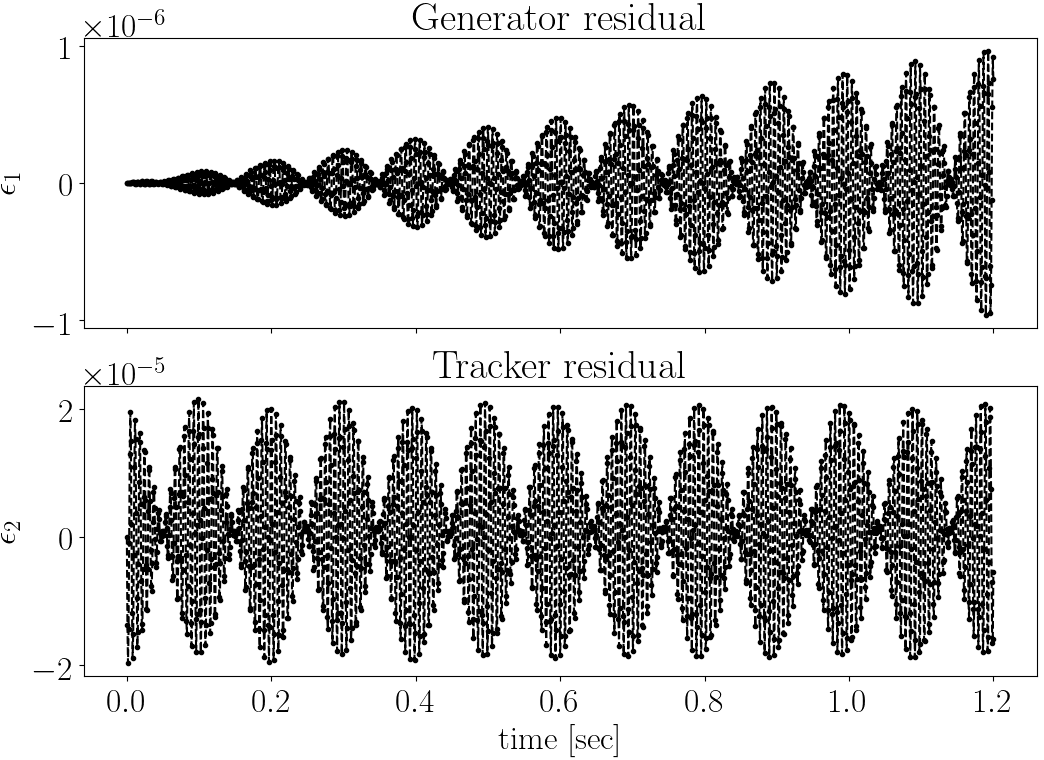
\includegraphics[height=.35\paperheight]{images/smp_sim/residual_vs_time(both)}
  \caption{Comparator residuals as functions of time.
    Top panel: $\epsilon_1$ residual; bottom panel: $\epsilon_2$ residual\label{fig:residuals}}
\end{figure}

\begin{figure}[h]
  \centering
  	\begin{subfigure}{\linewidth}
  		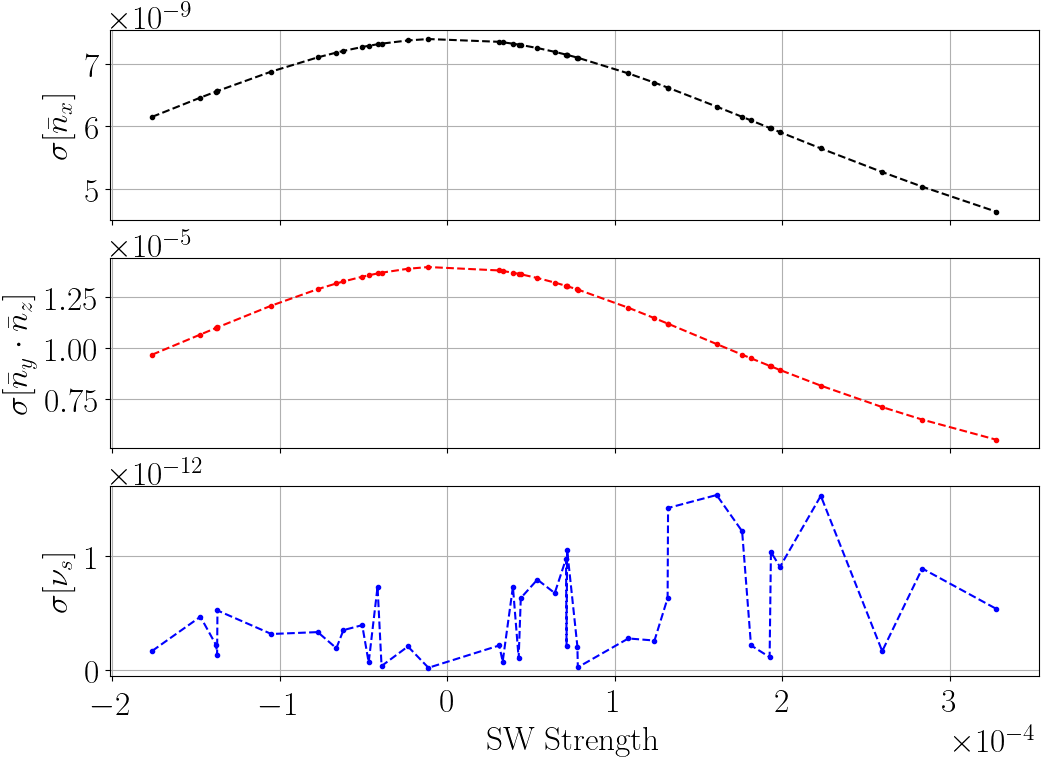
\includegraphics[height=.35\paperheight]{images/smp_sim/NBAR_variation_sd_vs_SW}
  		\caption{$\bar n$ component.\label{fig:sd:nbar}}
  	\end{subfigure}
	\begin{subfigure}{\linewidth}
		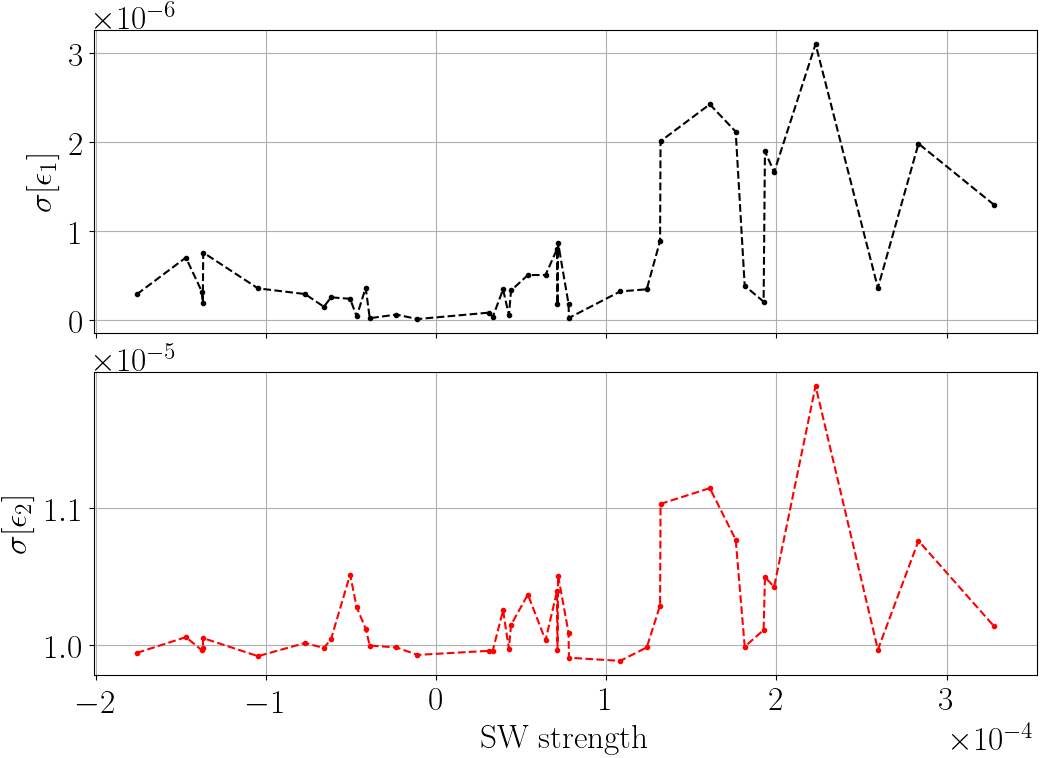
\includegraphics[height=.35\paperheight]{images/smp_sim/residual_SD_vs_SW(both)}
		\caption{Comparator residuals.
			Top panel: $\epsilon_1$ residual; bottom panel: $\epsilon_2$ residual\label{fig:sd:res}}
	\end{subfigure}
	\caption{Standard deviation vs spin wheel roll rate.\label{fig:sd}}
\end{figure}

\begin{table}[h]\centering
	\caption{Model parameter estimates (slow SW)\label{tbl:param_estimates}}
	\begin{tabular}{r|rllr}
		\hline
		Series & Par. & Value & St.Err & AIC \\
		\hline
		\multirow{3}{*}{$s_y^{idl}$}
		& $\hat f$ & 4.220359687911 & $6.9\cdot10^{-11}$ & \multirow{3}{*}{-62093} \\
		& $\hat a$ & 0.12514597851 & $4\cdot10^{-11}$ & \\
		& $\hat\delta$ & $-1.50\cdot10^{-8}$ & $4\cdot 10^{-10}$ &\\
		\hline
		\multirow{3}{*}{$s_y^{gen}$}
		& $\hat f$ & 4.2203596911 & $1.9\cdot 10^{-9}$ & \multirow{3}{*}{-52142} \\
		& $\hat a$ & 0.125145979 & $1\cdot 10^{-9}$ & \\
		& $\hat\delta$ & $-1.6\cdot 10^{-8}$ & $1.2\cdot 10^{-8}$ &\\
		\hline
		\multirow{3}{*}{$s_y^{trk}$}
		& $\hat f$ & 4.2203603 & $1.3\cdot 10^{-6}$ & \multirow{3}{*}{-34567} \\
		& $\hat a$ & 0.12514597 & $3.7\cdot10^{-7}$ & \\
		& $\hat\delta$ & $-4\cdot10^{-6}$ & $6\cdot 10^{-6}$ &\\
		\hline
	\end{tabular}
\end{table}


In Figure~\ref{fig:residuals} we observe that the ``generator'' is almost identical to the 
``ideal'' series, with $\epsilon_1 \le 1\cdot10^{-6}$ (even though its oscillation frequency is slightly off)
for the duration of the cycle, while the ``tracker'' series deviates from it at the level
$\epsilon_2 \le 2\cdot 10^{-5}$.  The discrepancy betweem $\epsilon_1$ and $\epsilon_2$ is observed
systematically at all spin wheel roll rates (see Figure~\ref{fig:sd:res}), and does not have an explanation
so far.

In Figure~\ref{fig:sd:res} we see that the standard deviations of both residuals exhibit the same dependence
on the spin wheel roll rate as that of $\nu_s$ (Figure~\ref{fig:sd:nbar}, bottom panel), but show indifference
toward the behavior of $\bar n$. This is an indication that frequency variation contributes a great deal more to the discrepance between model~\eqref{eq:fit_model} and the tracker data than the presumed amplitude variation
caused by the wobbling of $\bar n$ during betatron oscillations.

Table~\ref{tbl:param_estimates} characterized the model fit quality with respect to the used data set at the
slowest spin wheel roll rate. We observe that the cross-differences between the parameter estimates at different
time series are not statistically significant. Even though the variation of the spin precession angular velocity
dagraded the fit quality, it did not introduce any statistically-significant bias into the estimates.


\subsection{Conclusions}
The question of the influence of betatron motion on the EDM statistic in the FD method should be considered
in view of three circumstances:
\begin{enumerate}
\item The signal amplitude oscillations (as estimated by $\epsilon_2$) are small.
  They occur at the $10^{-4}$ level (when $\alpha\sim N(0, 3\cdot 10^{-2})$ degrees), whereas
  the expected polarization measurement error is on the order of percents.
  This means the superposition of this systematic error with the random measurement error
  will exhibit no statistically-significant systematicity.
\item The correllation coefficient between the amplitude and frequency estimates is not significant. The amplitude
  oscillations affect the $\hat a$-estimate foremost; their effect on the $\hat\w$-estimate is secondary, and is
  described by the correlation coefficient. Since it is less than 10\%, even if the oscillations happen to be
  strong enough to affect the amplitude estimate, their effect on the frequency estimate will be reduced by
  at least a factor of 10.
\item This systematic effect is controllable. And this point is the major advantage of the FD methodology.
  By applying an external Spin Wheel, the $\nbar$ oscillations can be continuously minimized
  as much as necessary, without changing the experiment pattern.
\end{enumerate}
